\documentclass[12pt]{article}
\usepackage[utf8x]{inputenc}
\usepackage{amsmath}
\usepackage{multicol}
\usepackage{graphicx}
\usepackage{float}
\usepackage{dsfont}
\usepackage{textcomp}
\usepackage{amsfonts}
\usepackage{cleveref}
\usepackage{fancyhdr}
\setlength{\headheight}{14.5pt}
\renewcommand{\sectionmark}[1]{\markright{#1}{}}
\usepackage[T1]{fontenc}
\usepackage[colorinlistoftodos]{todonotes}
\usepackage[margin=2.5cm,a4paper]{geometry}
\usepackage{listings}
\setlength{\marginparwidth}{2cm}
\setlength{\parindent}{0pt}
\newcommand{\deriv}{\mathrm{d}}
\lstset{
    language=R,
    basicstyle=\scriptsize\ttfamily,
    commentstyle=\ttfamily\color{red},
    numbers=left,
    numberstyle=\ttfamily\color{blue}\footnotesize,
    stepnumber=1,
    numbersep=5pt,
    backgroundcolor=\color{white},
    showspaces=false,
    showstringspaces=false,
    showtabs=false,
    frame=single,
    tabsize=2,
    captionpos=b,
    breaklines=true,
    breakatwhitespace=false,
    title=\lstname,
    escapeinside={},
    keywordstyle={},
    morekeywords={}
    }
\title{}
\pagestyle{fancy}
\fancyhf{}
\rhead{\leftmark}
\lhead{Exp.4 Gyroscopes}
\lfoot{PH520 Physics Laboratory A}
\rfoot{Page \thepage}
\renewcommand{\headrulewidth}{1pt}
\renewcommand{\footrulewidth}{1pt}
\begin{document}
\begin{titlepage}
\newgeometry{left=1.0in,right=1.0in,top=2.5in,bottom=2.5in}
\newcommand{\HRule}{\rule{\linewidth}{0.5mm}}
\begin{centering} 
%---------------------------------------------------------------------------
%	HEADING SECTIONS
%---------------------------------------------------------------------------

\includegraphics[scale=0.6]{Images/Uni_of_Kent.png}\\[1cm]
%---------------------------------------------------------------------------
%	TITLE SECTION
%---------------------------------------------------------------------------
\HRule \\[0.4cm]
\textsc{\large Astronomy, Space Science and Astrophysics}\\[0.5cm]
{ \Huge \bfseries Exp.4 Gyroscopes}\\[0.4cm]
\HRule \\[1.0cm]
%---------------------------------------------------------------------------
%	DATE SECTION
%---------------------------------------------------------------------------
\textsc{\Large PH520 - Stage 2}\\[0.5cm] 
\textsc{\Large Physics Laboratory A}\\[0.5cm] 
{\large Date: 21st Oct - 11th Nov 2019}\\[0.5cm]
%---------------------------------------------------------------------------
%	AUTHOR SECTION
%---------------------------------------------------------------------------
\begin{minipage}{0.625\textwidth}
\begin{center} \large
\emph{Report Author:} Lukasz R Tomaszewski \\[0.2cm]
\emph{Lab Partner:} Jessie Phillpot \\ [0.5cm]
{\large Word Count: 2414}\\
\end{center}
\end{minipage}\\[2cm]
\vfill
\end{centering} 
\end{titlepage}
%---------------------------------------------------------------------------
%	CONTENTS   
%---------------------------------------------------------------------------
\newpage
\begin{titlepage}
\begin{tableofcontents}
\end{tableofcontents}
\end{titlepage}
\newpage
%---------------------------------------------------------------------------
%	ABSTRACT
%---------------------------------------------------------------------------
\section{Abstract}
\label{Abstract Section}

This experiment proves the theoretical anticipations of the precession and the nutation of a gyroscope as its proved that the an external torque force directly affects how the pendulum/ gyroscope motion acts. It also shows that the angular frequency is directly related to the angular frequency of precession and nutation as the gyroscope is in motion and how the Sun and other celestial bodies affect the Earth’s rotation on its axis and why the North pole rotates every 26,000 years and causes "ice ages". Throughout this experiment, many errors arise as the human error take precedent due to reaction time set at +0.5s and the human manipulation of the speed of the torque that is induced upon the gyroscopes.

%---------------------------------------------------------------------------
%	INTRODUCTION
%---------------------------------------------------------------------------
\section{Introduction}
\label{Introduction Section}

“As this experiment observes rotational motion, the utilisation of newtons laws of torque and angular momentum will take effect as it shows how gyroscopes are formed and affected by multiple factors. This can be scaled to large masses such as planets and celestial objects, such as the Earth. The Earth rotates on its axis while orbiting the Sun, so as the Sun exerts a force upon Earth, other celestial bodies exert a torque that affects the Earth's angular momentum so as it presses, it causes a nutating rotation of its Northern pole every 26,000 years which causes "ice ages" to appear. Precesison of a gyroscope occurs when a applied torque cause the gyroscope to rotate in the same direction due to the weight of the spinning gyroscope, the torque is perpendicular to the angular momentum of the gyroscope. Nutation of a gyroscope occurs when the gyroscopes experiences precession and another small rotation takes place which is directly related to another external pushing/ pulling force.  ” \cite{Exp.4-2019} \\

%---------------------------------------------------------------------------
%	METHODOLOGY
%---------------------------------------------------------------------------
\section{Methodology}
\label{Methodology Section}
%---------------------------------------------------------------------------
\subsection{Theory}
\label{Theory Section}

Angular frequency \cite{Exp.4-2019}:
\begin{equation}
 \centering
 w = 2{\pi}f = \dfrac{2{\pi}}{{\Delta}t}n \hspace{0.1cm}
 \label{Angular Frequency Eq}
\end{equation} \\

Torque for a small angle \cite{Exp.4-2019}:
\begin{equation}
 \centering
 T = M_{wt}\hspace{0.1cm} g \hspace{0.1cm} sin{\theta} \hspace{0.1cm} R_{wt} \approx M_{wt} \hspace{0.1cm} g \hspace{0.1cm} {\theta} \hspace{0.1cm} R_{wt} = k_{wt} \hspace{0.1cm} \theta \hspace{0.1cm}\cite{Exp.4-2019}
 \label{Torque for a small angle Eq}
\end{equation} \\

Moment of Inertia of A1 Disk \cite{Exp.4-2019}:
\begin{equation}
 \centering
 I_{A1} = M_{wt}\hspace{0.1cm} R_{wt}\hspace{0.1cm} g\hspace{0.1cm} {\Delta}t^2/{4\pi^2}) - (M_{wt}\hspace{0.1cm} {R_{wt}}^2) \hspace{0.1cm}
 \label{Moment of Inertia of A1 Disk Eq}
\end{equation} \\

Useful Constants \cite{Exp.4-2019}:
\begin{table}[H]
\begin{center}
 \begin{math}
 \begin{tabular}{c c c}
 Parameter & Symbol & Value \\ 
 \hline
 Standard gravitational acceleration & g & $9.80665ms^{-2}$ \cite{Two} \\
 Mass of the gyroscope (inc. spindle) & $M_{Gyro}$ & (3.15 $\pm$0.01)kg \\
 Mass of A1 disk & $M_{A1}$ & (0.72955 $\pm$0.00002)kg\\
 \end{tabular}
 \end{math}
 \caption{Useful Constants. \cite{Exp.4-2019}}
 \label{Useful Constants}
\end{center}
\end{table}

%---------------------------------------------------------------------------
\subsection{Procedure}
\label{Procedure Section}
%---------------------------------------------------------------------------
\subsubsection{Moment of inertia of an aluminium disk}
\label{Moment of inertia of an aluminium disk method}

\textbf{\underline{Physical pendulum:}} \\

The apparatus was setup as shown in \cref{A1 Disk Setup}, the use of a vertically rod connected to a stand was used to elevate the aluminium disk that hung vertically off a horizontal rod connected via a multi-clamp to the bench clamp. The disk was then exposed to a torque from attaching two weights approx 100g each, and the mass of the screw and nut (all measured with a set of scales with a $\pm0.01g$ tolerance) at the base of the aluminium disk. Note that the horizontal rod suspending the disk and the weights attached to the disk are opposite each other at each opposite edge of the A1 disk at a distance R (to be measured with a ruler with a $\pm0.01cm$ tolerance). By moving the weights thus creating a small angle, a torque was formed, thus the period was repeatedly measured and an average value was formed as the period ${\Delta}t$ timed via a stopwatch with a $\pm0.01s$ tolerance while factoring in a reaction time at +0.5, thus allowing the moment of inertia for the A1 disk \cref{Moment of Inertia of A1 Disk Eq} to be determined. \\ 

\begin{figure}[H]
\centering
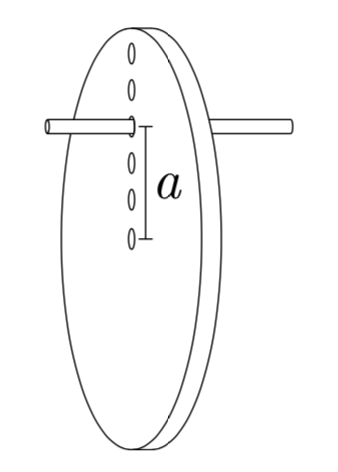
\includegraphics[scale=0.6]{Images/Labscript/Steiners_Law_A1_Disk.png}
\caption{A1 disk setup for measuring moment of inertia. \cite{Exp.4-2019}}
\label{A1 Disk Setup}
\end{figure}

\textbf{\underline{Steiner's law:}} \\

Utilizing the same setup in \cref{A1 Disk Setup}, the d $\approx$ 4cm spaced holes on the aluminium disk were measured with the vernier with a $\pm0.01cm$ tolerance, the same weights, screw and nut (all measured with a set of scales with a $\pm0.01g$ tolerance) were added to the edge of the aluminium disk, the horizontal rod suspending the disk was moved into the centre of the disk. By applying the disk with a small angle by shifting the weights to one side to provide a torque, this was repeated 3 times and the distance between the horizontal support and the weights measured at 0cm to 16cm in of 4cm increments by moving the horizontal rod to each pre-cut hole. The period of these pendulum swings is measured by a stopwatch with a $\pm$0.01s error while factoring in a reaction time at +0.5s, the physical data of the period can be compared with the theoretical data. \\

%---------------------------------------------------------------------------
\subsubsection{Precession of a gyroscope}
\label{Precession of a gyroscope method}

\textbf{\underline{Moment of inertia:}} \\

By setting the gyroscope vertically supported by a horizontal rod connected to a stand, a infrared sensor is supported via a bench clamp that is connected to a digital counter and is placed so that the gyroscope is in between the two sensors so that the sensors can count the spokes of the gyroscope as seen in \cref{2.1 Moment of Inertia Setup} so that the period of the spinning gyroscope can be determined. At the base of the the gyroscopes, two weights, nut and bolt (all measured with a set of scales with a $\pm0.01g$ tolerance) are hung to provide a torque so when a small angle is induced, the gyroscope is subject to a pendulum motion. This motion will produce a period to which will be measured via the digital counter with a $\pm$0.001 error, this is repeated 5 times and an average value is deduced. \\

\begin{figure}[H]
\centering
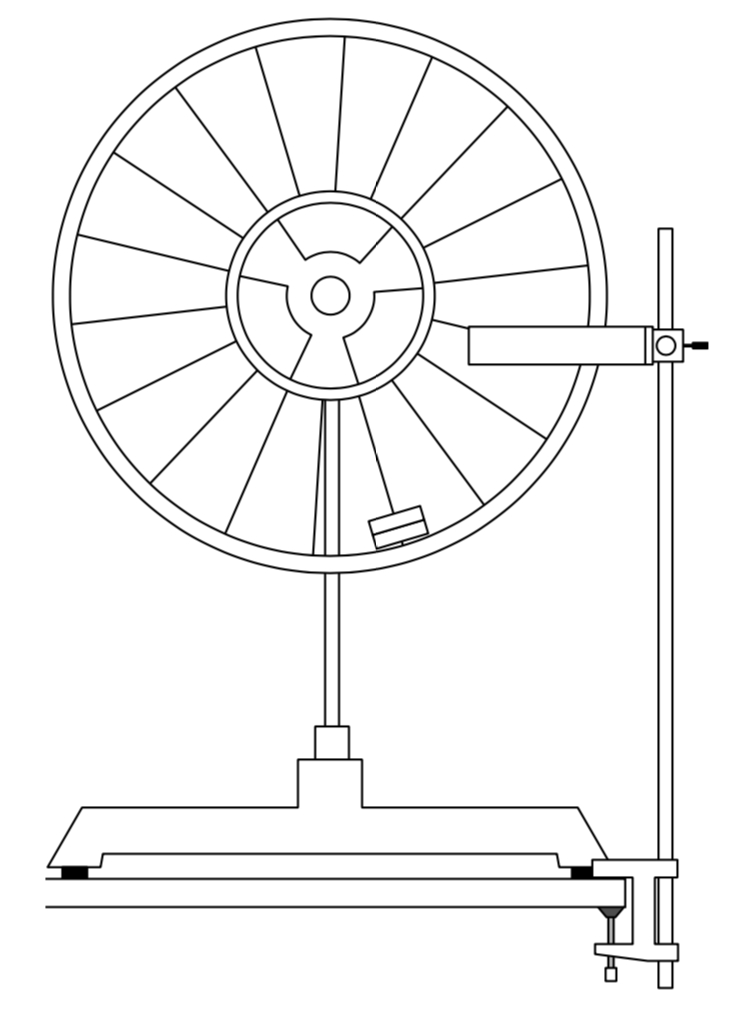
\includegraphics[scale=0.5]{Images/Labscript/21_Moment_Of_Inertia.png}
\caption{Setup of the gyroscope to form a physical pendulum. \cite{Exp.4-2019}}
\label{2.1 Moment of Inertia Setup}
\end{figure} 

\textbf{\underline{Centre of gravity:}} \\

Suspending the gyroscope horizontally on a vertical rod connected to a stand as shown in \cref{2.2 Center of Gravity Setup} and thus changing the gyroscopes support pole height $s$ as seen in \cref{Center of gravity height Setup} by using an hex key to loosen and tighten a pin that secures the gyroscope to the support pole. The centre of gravity can be found when the gyroscope is perfectly balanced on the vertical rod and when subject to an external force will return to is original position. The use of the vernier caliper is to measure the distance $s (s_0+d)$ shown on \cref{Center of gravity height Setup} with a tolerance of $\pm0.01cm$. \\

\begin{multicols}{2}
\begin{figure}[H]
\centering
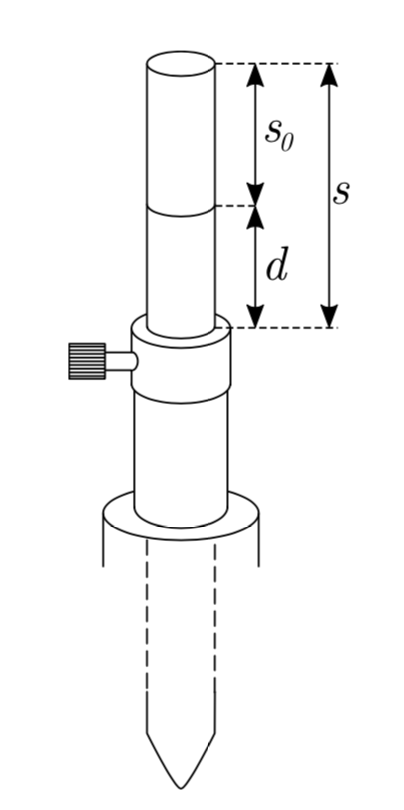
\includegraphics[scale=0.545]{Images/Labscript/Gyroscope_Rod.png}
\caption{Changing the height of the gyroscope to find the centre of gravity \cite{Exp.4-2019}}
\label{Center of gravity height Setup}
\end{figure}

\begin{figure}[H]
\centering
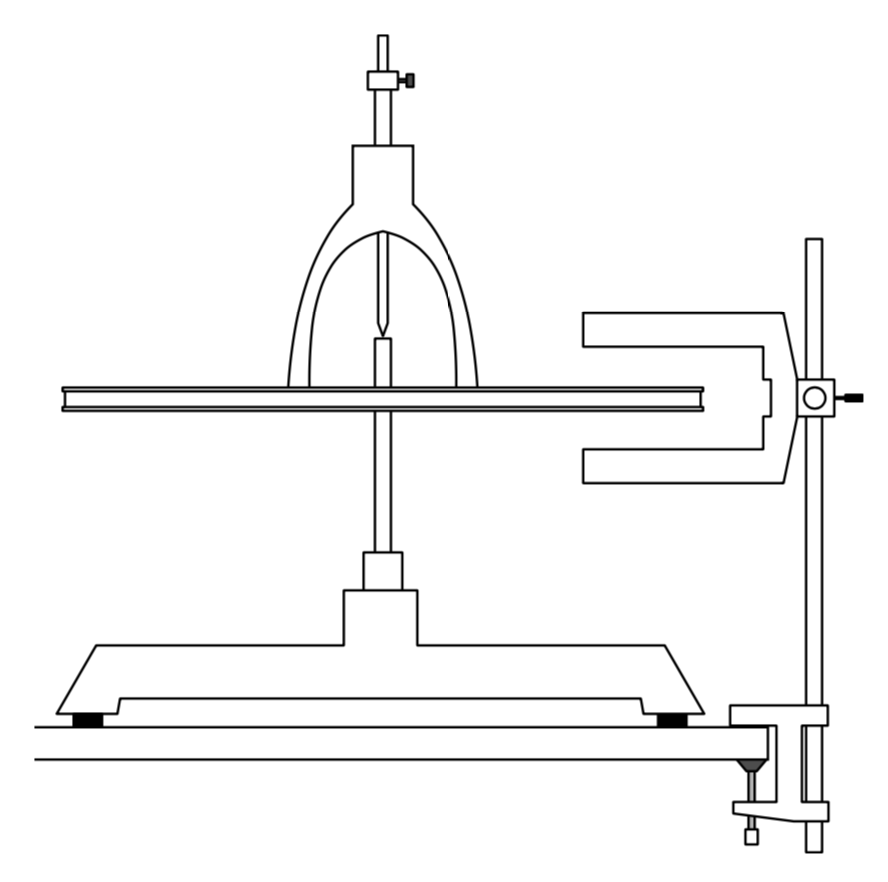
\includegraphics[scale=0.5]{Images/Labscript/22_Centre_of_Gravity.png}
\caption{Setup of the gyroscope to find its centre of gravity. \cite{Exp.4-2019}}
\label{2.2 Center of Gravity Setup}
\end{figure}
\end{multicols}

\textbf{\underline{Precession:}} \\

By finding the centre of gravity of the gyroscope, by suspending the gyroscope via its support pole horizontally on a vertical rod shown in \cref{2.2 Center of Gravity Setup}, the gyroscope is in a state of equilibrium. To find the precession, the height of the support pole must be altered, by changing $s (s_0+d)$ in \cref{Center of gravity height Setup} by $\pm3cm$ in 1cm increments (measured with vernier calipers with a $\pm0.01cm$ tolerance) allows a variable rate of precession to take place. \\

\begin{figure}[H]
\centering
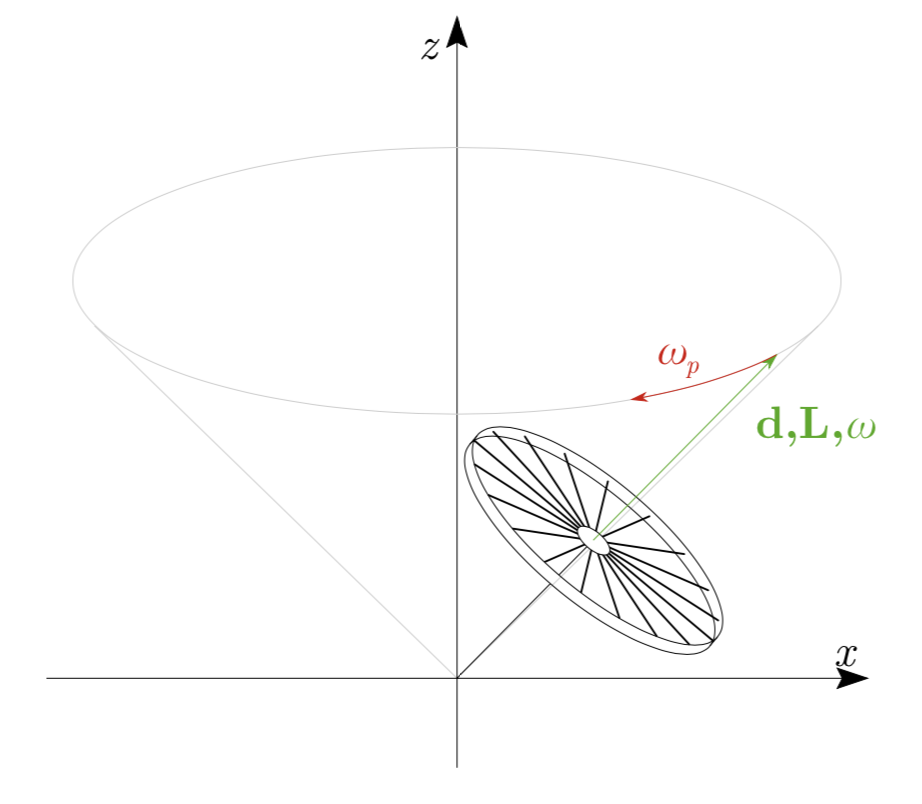
\includegraphics[scale=0.5]{Images/Labscript/Gyroscope_Precession.png}
\caption{Diagram showing the precession of the gyroscope. \cite{Exp.4-2019}}
\label{Precession of the gyroscope Setup}
\end{figure} 

By placing the infrared sensor so that it can count the spokes of the gyroscope and connect the infrared sensor to the digital counter, the precession can be measured. By spinning the gyroscope at the different heights, precession takes place upon the gyroscope where the digital counter counts the frequency of the gyroscopes time period (rotation) with a $\pm0.001s$ tolerance and the stopwatch is used to measure the top of the gyroscope as it makes a complete rotation with a $\pm0.01s$ tolerance as the gyroscope will now spin of an angled axis and will slowly rotate, this is precession. With the values recorded, the angular frequency and angular frequency of precession shown in \cref{Precession of the gyroscope Setup} can be determined. \\

\subsubsection{Nutation of a gyroscope}
\label{Nutation of a gyroscope method}

By utilizing the set up shown in \cref{2.2 Center of Gravity Setup} where the gyroscope sits horizontal suspending of its support pole on a vertical rod connected to a stand, with the infrared sensor positioned so which its sensors can measure the spokes of the gyroscope, with the infrared sensor connected to the digital counter. By changing the height of the gyroscopes support pole $s (s_0+d)$ in \cref{Center of gravity height Setup} to find the centre of gravity, once found, with the gyroscope spinning a small vertical external force is applied to allow nutation of the gyroscope to take place, where the gyroscope 3 rotational motions are taking place as shown in \cref{Nutation of the gyroscope Setup}. \\

\begin{figure}[H]
\centering
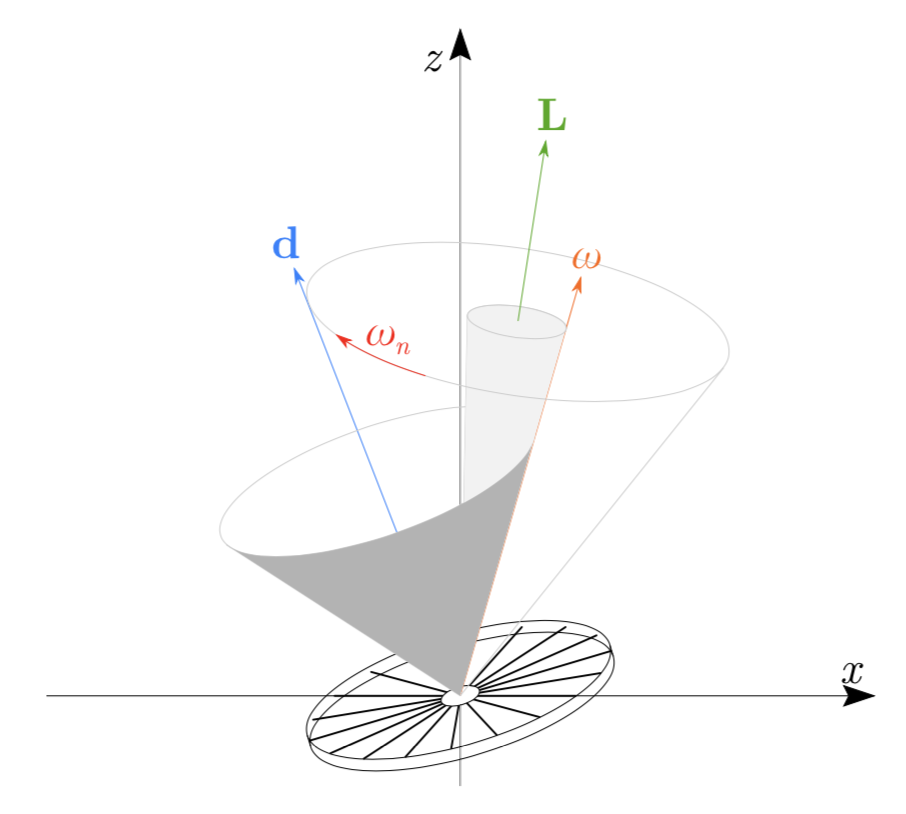
\includegraphics[scale=0.6]{Images/Labscript/Gyroscope_Nutation.png}
\caption{Diagram showing the nutation of the gyroscope. \cite{Exp.4-2019}}
\label{Nutation of the gyroscope Setup}
\end{figure}

With the digital counter set to count the frequency of the gyroscopes time period (rotation) with a $\pm0.001s$ tolerance and the stopwatch is used to measure the top of the gyroscope with a $\pm0.01s$ tolerance as it makes a complete rotation $w$. $w_n$ can then be calculate and compared with $w$ and relationship can formed.

%---------------------------------------------------------------------------
%	REPORT & FINDINGS
%---------------------------------------------------------------------------
\section{Results \& Findings}
\label{Results & findings Section}
%---------------------------------------------------------------------------
\subsection{Moment of inertia of an aluminium disk}
\label{Moment of inertia of an aluminium disk Findings}
%---------------------------------------------------------------------------
\subsubsection{Physical pendulum}
\label{Physcial Pendulum Findings}

Starting with a simple pendulum set up utilising the A1 disk shown in \cref{A1 Disk Setup}, the total mass of the two weights, screw and nut measured to be 195.84g with the mass of the screw taken into effect shown in \cref{Values of the total mass of the weights and pendulum table}. By setting the distance between the horizontal support point and the weights at 16.2cm $\pm0.1cm$. There is no way to accurately measure the angle that was induced but the angle doesn't affect the period of the pendulum, the period of the pendulum is directly related to the length of the pendulum $R_{wt}$ and the mass at the base of the pendulum $M_{wt}$. \\

\begin{table}[H]
\begin{center}
 \footnotesize
 \begin{tabular}{|c||c|c|c|c|c|}
 \hline
 \multicolumn{6}{|c|}{Total mass of the weights and pendulum} \\
 \hline \hline
  & Mass 1 & Mass 2 & Mass 3 & Avg. Mass & Error (g) \\
 \hline
 Mass of Weight 1 (g) & 96.36 & 96.37 & 96.37 & 96.37 & $\pm$0.01g \\
 \hline
 Mass of Weight 2 (g) & 95.84 & 95.85 & 95.84 & 95.84 & $\pm$0.01g \\
 \hline
 Mass of Screw/Nut (g) & 3.63 & 3.63 & 3.63 & 3.63 & $\pm$0.01g \\
 \hline \hline
 Total Mass (g) &&&& 195.84 & $\pm$0.03g \\
 \hline \hline
 Mass of A1 Disk (g) &&&& 729.55 & $\pm$0.02g \\
 \hline
 \end{tabular}
 \caption{Values of the total mass of the weights and pendulum}
 \label{Values of the total mass of the weights and pendulum table}
\end{center}
\end{table}

\begin{table}[H]
\begin{center}
 \footnotesize
 \begin{tabular}{|c||c|c|c|c|c|c|c|}
 \hline
 \multicolumn{8}{|c|}{Period of the physical pendulum} \\
 \hline \hline
  & 1 & 2 & 3 & 4 & 5 & Avg. Time & Error (s) \\
 \hline
 $\Delta$T (s) & 1.19 & 1.15 & 1.10 & 1.13 & 1.21 & 1.156 & $0.01$s \\
 \hline
 \end{tabular}
 \caption{Values of the period of the physical pendulum}
 \label{Values of the period of the physical pendulum table}
\end{center}
\end{table}

Moment of Inertia of A1 Disk:
By converting all measurements into SI units so that \cref{Moment of Inertia of A1 Disk Eq} can be determined
\begin{equation}
 \centering
 I_{A1} = \dfrac{0.19584kg\hspace{0.1cm} 0.162m\hspace{0.1cm} 9.80665ms^{-2}\hspace{0.1cm} 1.156s^2}{4{\pi}^2} - (0.19584kg\hspace{0.1cm} 0.162m^2) = 0.005392kgm^{-2}
 \label{Moment of Inertia of A1 Disk Eq Ans}
\end{equation} \\

\textbf{\underline{Errors Analysis}}: \\
\begin{table}[H]
\begin{center}
 \begin{math}
 \begin{tabular}{c c c}
 Distance (r)  = & $\pm$0.001m \\
 Stopwatch (s) = & $\pm$0.01s \\
 Weights (g) = & $\pm$0.01g \\ \\
 Sample SD : ${\Delta}t$: 0.044497 \\
 Error : ${\Delta}t$: ${\pm}$0.0205 \\
 Total Error : ${\Delta}t$: 1.16 ${\pm}$0.0205 \\
 \end{tabular}
 \end{math}
 
 \caption{Physical Pendulum Error Analysis.}
 \label{1.1 Error Analysis}
\end{center}
\end{table}

%---------------------------------------------------------------------------
\subsubsection{Steiner's Law}
\label{Steiners Law Findings}

Utilizing the setup from \cref{A1 Disk Setup}, it was found that increasing the length of the pendulum directly affects the period of the pendulum. The induced angle doesn't doesn't affect the period of the pendulum and thus is irrelevant, only the length and mass affects the period of the pendulum. As physics implies a heavier mass and longer length increases the period of the pendulum motion. In \cref{Values of the period of the physical pendulum Steiners table}, its seen that this is not the case, the increase of length slows the pendulum motion  down not increases as theory would suggest. The only reasoning behind this is the reaction time of the human operators that are operating the stopwatch, which means the time can be $\pm0.5s$ faster/ slower as the operator tried to for see the time the pendulum motion had completed its swing and thus creating small but vital errors in the calculations. From these values the moment of inertia is calculated as shown in \cref{1.2 Theory}.   \\

\begin{table}[H]
\begin{center}
 \footnotesize
 \begin{tabular}{|c||c|c|c|c|c|c|c|c|}
 \hline
 \multicolumn{8}{|c|}{Precession of the physical pendulum} \\
 \hline \hline
 & & 1 & 2 & 3  & Avg. Time & Error (s) & Error (cm) \\
 \hline
 0cm & $\Delta$T(s) & 0 & 0 & 0 & 0 & 0 & 0 \\
 \hline
 4cm & $\Delta$T(s) & 1.19 & 1.12 & 0.94 & 1.08 & $\pm$0.01s & $\pm$0.01cm \\
 \hline
 8cm & $\Delta$T(s) & 0.87 & 0.78 & 0.90 & 0.85 & $\pm$0.01s & $\pm$0.01cm \\
 \hline
 12cm & $\Delta$T(s) & 0.87 & 0.78 & 0.81 & 0.82 & $\pm$0.01s & $\pm$0.01cm \\
 \hline
 16cm & $\Delta$T(s) & 0.94 & 0.81 & 0.87 & 0.87 & $\pm$0.01s & $\pm$0.01cm \\
 \hline
 \end{tabular}
 \caption{Values of the period of the physical pendulum}
 \label{Values of the period of the physical pendulum Steiners table}
\end{center}
\end{table}

\begin{table}[H]
\begin{center}
 \footnotesize
 \begin{tabular}{|c||c|c|c|c|c|}
  \hline
 \multicolumn{6}{|c|}{Moment of Inertia Calculated vs Theoretical Results} \\
 \hline \hline
  Distance (cm) & 0 & 4 & 8 & 12 & 16\\
 \hline \hline
  Actual ${\Delta}t$ & 0 & 0.00196 & 0.00158 & 0.00111 & 0.00088 \\
 \hline
  Theoretical ${\Delta}t$ & 0 & 0.00729 & 0.00581 & 0.00412 & 0.00327 \\
 \hline
 \end{tabular}
 \caption{Moment of Inertia Calculated vs Theoretical Results.}
 \label{1.2 Theory}
\end{center}
\end{table}

\textbf{\underline{Errors Analysis}}: \\
\begin{table}[H]
\begin{center}
 \begin{math}
 \begin{tabular}{c c c}
 Distance (r)  = & $\pm$0.001m \\
 Stopwatch (s) = & $\pm$0.01s \\
 Weights (g) = & $\pm$0.01g \\ \\
 \end{tabular}
 \end{math}
 \caption{Steiner's Law Error Analysis.}
 \label{1.2 Error Analysis}
\end{center}
\end{table}

\begin{table}[H]
\begin{center}
 \footnotesize
 \begin{tabular}{c c c c c c}
 & 0cm &4cm & 8cm & 12cm & 16cm \\
 Sample SD: $\Delta$T(s): & 0 & 0.12897 & 0.06245 & 0.045826 & 0.065064\\
 Error: $\Delta$T(s): & 0 & $\pm$0.07 & $\pm$0.04 & $\pm$0.03 & $\pm$0.04 \\
 Total Error: $\Delta$T(s): & 0 & 1.08 $\pm$0.07 & 0.85 $\pm$0.04 & 0.82 $\pm$0.03 & 0.87 $\pm$0.04 \\
 \end{tabular}
 \caption{Steiner's Law Error Analysis.}
 \label{1.2 Error Analysis SD}
\end{center}
\end{table}

%---------------------------------------------------------------------------
\subsubsection{Moment of Inertia of a Gyroscope}
\label{Moment of Inertia of a Gyroscope Findings}

By using the gyroscope and placing the weights at the base of the gyroscope with the combined mass of 195.84g $\pm0.01g$ proved in \cref{Values of the total mass of the weights and pendulum table} and the distance between the weights and the horizontal support point set at 23.9cm $\pm0.011cm$. Using the the average time of the repeatedly measured results, the moment of inertia can be determined by using \cref{Moment of Inertia of A1 Disk Eq}.

\begin{table}[H]
\begin{center}
 \footnotesize
 \begin{tabular}{|c||c|c|c|c|c|c|c|}
 \hline
 \multicolumn{8}{|c|}{Period of the gyroscope} \\
 \hline \hline
  & 1 & 2 & 3 & 4 & 5 & Avg. Time & Error (s) \\
 \hline
 $\Delta$T (s) & 3.47 & 3.31 & 3.35 & 3.41 & 3.38 & 3.38 & $\pm$0.01s \\
 \hline
 \end{tabular}
 \caption{Period of the gyroscope}
 \label{Period of the gyroscope table}
\end{center}
\end{table}

Moment of Inertia of A1 Disk:
By converting all measurements into SI units so that \cref{Moment of Inertia of A1 Disk Eq} can be determined
\begin{equation}
 \centering
 I_{A1} = \dfrac{0.19584kg\hspace{0.1cm} 0.239m\hspace{0.1cm} 9.80665ms^{-2}\hspace{0.1cm} 3.38s^2}{4{\pi}^2} - (0.19584kg\hspace{0.1cm} 0.239m^2) = 0.122kgm^{-2}
 \label{Moment of Inertia of gyroscope Ans}
\end{equation} \\

\textbf{\underline{Errors Analysis}}: \\
\begin{table}[H]
\begin{center}
 \begin{math}
 \begin{tabular}{c c c}
 Distance (r)  = & $\pm$0.001m \\
 Stopwatch (s) = & $\pm$0.01s \\
 Weights (g) = & $\pm$0.01g \\ \\
 \end{tabular}
 \end{math}
 \caption{Moment of Inertia Error Analysis.}
 \label{2.1 Error Analysis}
\end{center}
\end{table}

%---------------------------------------------------------------------------
\subsubsection{Centre of Gravity}
\label{Centre of Gravity Findings}

By using the vernier callipers the centre of gravity was found by changing $d$ in \cref{Center of gravity height Setup}, its found that the centre of gravity was at $s=9.96cm$ $\pm0.01cm$. It was confirmed the be the centre of gravity by applying a small force on the gyroscope, the gyroscope then returned to a flat stationary position where $F=0$. 

%---------------------------------------------------------------------------
\subsubsection{Precession of a Gyroscope}
\label{Precession of a Gyroscope Findings}

As the gyroscope is at its centre of gravity, there cannot be any precession, to find the precession $s$ is changed in \cref{Center of gravity height Setup} in reference to the centre of gravity. The results shown in \cref{Precession of a gyroscope table} tell the further away from the centre of gravity the gyroscope sits, the more precession is obtained. Using this to explore how the Earth experiences precession around the Sun, as the Suns forces causes the Earth to rotate allowing the Earth to endure a daytime and nighttime per a 24hr clock system. \\

\begin{table}[H]
\begin{center}
 \footnotesize
 \begin{tabular}{|c||c|c|c|c|c|c|c|c|}
 \hline
 \multicolumn{9}{|c|}{Precession of a gyroscope} \\
 \hline \hline
 Distance (cm) & $\Delta$T (s) & $\Delta$$T_p$ (s) & $\Delta$T/18 (s) & $w$ (Hz) & $w_p$ (Hz) & Error (s) & Error (cm) & Error (Hz)\\
 \hline \hline
 1cm  & 0.044 & 14.53 & 0.792 & 9.93 & 0.43 & $\pm$0.01s & $\pm$0.01g & $\pm$0.02Hz\\
 \hline
 1cm  & 0.043 & 15.30 & 0.774 & 8.12 & 0.41 & $\pm$0.01s & $\pm$0.01g & $\pm$0.02Hz\\
 \hline
 1cm  & 0.045 & 15.63 & 0.810 & 7.76 & 0.40 & $\pm$0.01s & $\pm$0.01g & $\pm$0.02Hz \\
 \hline
 2cm  & 0.049 & 9.10 & 0.882 & 7.12 & 0.69 & $\pm$0.01s & $\pm$0.01g& $\pm$0.02Hz \\
 \hline
 3cm  & 0.045 & 8.09 & 0.810 & 7.76 & 0.78 & $\pm$0.01s & $\pm$0.01g & $\pm$0.02Hz\\
 \hline \hline
 -1cm  & 0.040 & 22.44 & 0.720 & 8.73 & 0.28 & $\pm$0.01s & $\pm$0.01g & $\pm$0.02Hz\\
 \hline
 -2cm  & 0.038 & 13.41 & 0.684 & 9.19 & 0.47 & $\pm$0.01s & $\pm$0.01g & $\pm$0.02Hz\\
 \hline
 -3cm  & 0.038 & 8.84 & 0.702 & 8.95 & 0.71 & $\pm$0.01s & $\pm$0.01g & $\pm$0.02Hz\\
 \hline
 \end{tabular}
 \caption{Precession of a gyroscope}
 \label{Precession of a gyroscope table}
\end{center}
\end{table}

\begin{multicols}{2}
\begin{figure}[H]
\centering
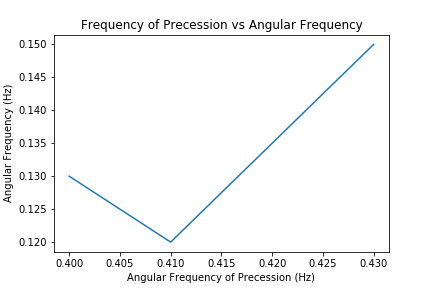
\includegraphics[scale=0.6]{Images/StillAngularFrequencyvsFrequencyofPrecession.png}
\caption{The relationship between angular frequency $w$ and angular frequency of precession $w_p$.}
\label{Still precesison}
\end{figure}

\begin{figure}[H]
\centering
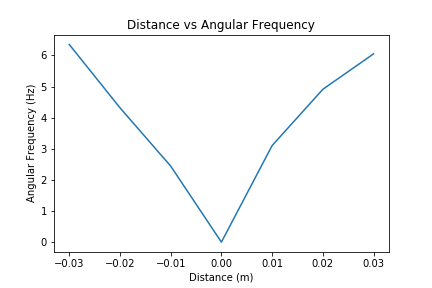
\includegraphics[scale=0.6]{Images/ChangeAngularFrequencyvsFrequencyofPrecession.png}
\caption{The relationship between angular frequency $w$ and distance $s$.}
\label{change precession}
\end{figure}
\end{multicols}

By plotting the angular frequency against the angular frequency of precession in \cref{Still precesison} and distance \cref{change precession}, relationships can be seen. In \cref{Still precesison} where the distance did not change over 3 measurements, it shows that as angular frequency rises so does the angular frequency of precession, the only error in this is in the second measurement, but the human error factor is taken into account. When changing the distance in \cref{change precession} no matter the increase of distance from the centre of gravity whether its direction is positive or negative, the angular frequency increases steadily according to the increase in length. \\

Exploring further, the precession of the gyroscope is subject to human error as the human operators reaction time is $+0.5s$ on the stopwatch time ${\Delta}t$ this is consecutive across all of the measurements and is therefore equal throughout the results as every value experiences this. \\

\textbf{\underline{Errors Analysis}}: \\
\begin{table}[H]
\begin{center}
 \begin{math}
 \begin{tabular}{c c c}
 Distance (r)  = & $\pm$0.001m \\
 Stopwatch (s) = & $\pm$0.01s \\
 Weights (g) = & $\pm$0.01g \\ \\
 \end{tabular}
 \end{math}
 \caption{Precession of a Gyroscopes Error Analysis.}
 \label{2.2 Error Analysis}
\end{center}
\end{table}

%---------------------------------------------------------------------------
\subsection{Nutation of a Gyroscope}
\label{Nutation of a Gyroscope Findings}

By moving the gyroscope into its centre of gravity by changing $s$ in \cref{Center of gravity height Setup} so that $s=4.0cm$ $\pm0.01cm$ the nutation can be measured and $w$ \& $w_n$ are calculated using \cref{Angular Frequency Eq}.

\begin{table}[H]
\begin{center}
 \footnotesize
 \begin{tabular}{|c||c|c|c|c|c||c|c|c|}
 \hline
 \multicolumn{9}{|c|}{Nutation of a gyroscope} \\
 \hline \hline
  & ${\Delta}t/18$ (s) & $s{\Delta}t_n$ (s) & ${\Delta}t$ (s) & ${\Delta}t_n$ (s) & Error (s) & $w$ (Hz) & $w_n$ (Hz) & Error (Hz)\\
 \hline \hline
 1  & 0.051 & 3.00 & 0.918 & 0.600 & $\pm$0.01s & 6.84 & 10.47 & $\pm$0.02Hz \\
 \hline
 2  & 0.035 & 2.06 & 0.630 & 0.412 & $\pm$0.01s & 9.97 & 15.25 & $\pm$0.02Hz \\
 \hline
 3  & 0.027 & 1.53 & 0.306 & 0.306 & $\pm$0.01s & 12.93 & 20.53 & $\pm$0.02Hz \\
 \hline
 \end{tabular}
 \caption{Nutation of a gyroscope}
 \label{Nutation of a gyroscope table}
\end{center}
\end{table}

Taking all the relevant measurements shown in \cref{Nutation of a gyroscope table} allows a relationship to be seen between $w$ and $w_n$. It can be seen in \cref{Nutation comparison} that the angular frequency of nutation is always greater than the angular frequency and as the angular frequency increases the angular frequency of nutation steadily increases also proving that the angular frequency of nutation is directly related to the angular frequency. When applying a force down onto the rotating gyroscope to cause nutation to occur, that force is caused by human manipulation and cannot be accurately measured and directly affects the time period $s{\Delta}t_n$.\\

\begin{figure}[H]
\centering
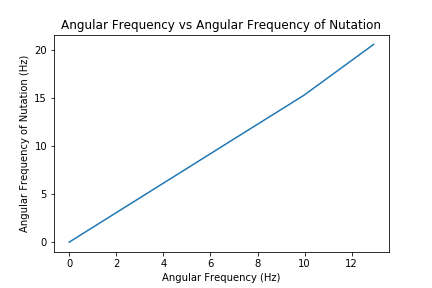
\includegraphics[scale=0.6]{Images/AngularFrequencyvsFrequencyofNutation.png}
\caption{The relationship between angular frequency $w$ and angular frequency of nutation $w_n$.}
\label{Nutation comparison}
\end{figure}

\textbf{\underline{Errors Analysis}}: \\
\begin{table}[H]
\begin{center}
 \begin{math}
 \begin{tabular}{c c c}
 Distance (r)  = & $\pm$0.001m \\
 Stopwatch (s) = & $\pm$0.01s \\
 Weights (g) = & $\pm$0.01g \\
 \end{tabular}
 \end{math}
 \caption{Nutation of a Gyroscope Error Analysis.}
 \label{3 Error Analysis}
\end{center}
\end{table}

%---------------------------------------------------------------------------
%	DISCUSSION
%---------------------------------------------------------------------------
\section{Discussion}
\label{Disscussion Section}

Within this experiment, its seen that the torque directly affects the angular momentum of the gyroscope but it encounters a variety of errors, human error plays throughout this experiment as all the time periods are measured with a stopwatch and the human operator must manually press the start and stop button, therefore a reaction time from when the stopwatch is started and stop to when the pendulum/ gyroscope is released and completed one measurable motion was set at $+0.5s$. It's also seen that the length of the pendulum affected the time period shown in \cref{Physcial Pendulum Findings}, when the theoretical data tells otherwise, when the only error that could be accountable for this is human error by the operators anticipating the end of the pendulums motion to early and stopping the stopwatch earlier than it needed to be. \\

%---------------------------------------------------------------------------
%	CONCLUSION
%---------------------------------------------------------------------------
\section{Conclusion}
\label{Conclusion Section}

Its clear to see that the precession and the nutation are affected by external forces such as a torque, this allows the exploration of how the Earth's rotation is affected by the Sun and other celestial objects. This is proved in \cref{Precession of a Gyroscope Findings} where in \cref{change precession} where the distance from the centre of gravity increases, the angular frequency increases from the torque force that is enforced upon the gyroscope. Its also proved in \cref{Nutation of a Gyroscope Findings} where in \cref{Nutation comparison} shows that as the angular frequency increases so does the angular frequency of nutation, thus shows that as with Earth's radius, the radius also being the distance from the centre of gravity it shows that the Suns causes a torque force upon the Earth and causes it to precess whereas other celestial bodies also affect the Earths rotation by applying their external forces upon it and cause the Earth to undergo nutation thus explaining why the earths north pole rotates every 26,000 years and why "ice ages" occur. \\

%---------------------------------------------------------------------------
%	REFERENCES
%---------------------------------------------------------------------------
\bibliographystyle{plain}
\bibliography{mybib.bib}
\end{document}